\documentclass[twoside]{book}

% Packages required by doxygen
\usepackage{fixltx2e}
\usepackage{calc}
\usepackage{doxygen}
\usepackage[export]{adjustbox} % also loads graphicx
\usepackage{graphicx}
\usepackage[utf8]{inputenc}
\usepackage{makeidx}
\usepackage{multicol}
\usepackage{multirow}
\PassOptionsToPackage{warn}{textcomp}
\usepackage{textcomp}
\usepackage[nointegrals]{wasysym}
\usepackage[table]{xcolor}

% Font selection
\usepackage[T1]{fontenc}
\usepackage[scaled=.90]{helvet}
\usepackage{courier}
\usepackage{amssymb}
\usepackage{sectsty}
\renewcommand{\familydefault}{\sfdefault}
\allsectionsfont{%
  \fontseries{bc}\selectfont%
  \color{darkgray}%
}
\renewcommand{\DoxyLabelFont}{%
  \fontseries{bc}\selectfont%
  \color{darkgray}%
}
\newcommand{\+}{\discretionary{\mbox{\scriptsize$\hookleftarrow$}}{}{}}

% Page & text layout
\usepackage{geometry}
\geometry{%
  a4paper,%
  top=2.5cm,%
  bottom=2.5cm,%
  left=2.5cm,%
  right=2.5cm%
}
\tolerance=750
\hfuzz=15pt
\hbadness=750
\setlength{\emergencystretch}{15pt}
\setlength{\parindent}{0cm}
\setlength{\parskip}{3ex plus 2ex minus 2ex}
\makeatletter
\renewcommand{\paragraph}{%
  \@startsection{paragraph}{4}{0ex}{-1.0ex}{1.0ex}{%
    \normalfont\normalsize\bfseries\SS@parafont%
  }%
}
\renewcommand{\subparagraph}{%
  \@startsection{subparagraph}{5}{0ex}{-1.0ex}{1.0ex}{%
    \normalfont\normalsize\bfseries\SS@subparafont%
  }%
}
\makeatother

% Headers & footers
\usepackage{fancyhdr}
\pagestyle{fancyplain}
\fancyhead[LE]{\fancyplain{}{\bfseries\thepage}}
\fancyhead[CE]{\fancyplain{}{}}
\fancyhead[RE]{\fancyplain{}{\bfseries\leftmark}}
\fancyhead[LO]{\fancyplain{}{\bfseries\rightmark}}
\fancyhead[CO]{\fancyplain{}{}}
\fancyhead[RO]{\fancyplain{}{\bfseries\thepage}}
\fancyfoot[LE]{\fancyplain{}{}}
\fancyfoot[CE]{\fancyplain{}{}}
\fancyfoot[RE]{\fancyplain{}{\bfseries\scriptsize Generated by Doxygen }}
\fancyfoot[LO]{\fancyplain{}{\bfseries\scriptsize Generated by Doxygen }}
\fancyfoot[CO]{\fancyplain{}{}}
\fancyfoot[RO]{\fancyplain{}{}}
\renewcommand{\footrulewidth}{0.4pt}
\renewcommand{\chaptermark}[1]{%
  \markboth{#1}{}%
}
\renewcommand{\sectionmark}[1]{%
  \markright{\thesection\ #1}%
}

% Indices & bibliography
\usepackage{natbib}
\usepackage[titles]{tocloft}
\setcounter{tocdepth}{3}
\setcounter{secnumdepth}{5}
\makeindex

% Hyperlinks (required, but should be loaded last)
\usepackage{ifpdf}
\ifpdf
  \usepackage[pdftex,pagebackref=true]{hyperref}
\else
  \usepackage[ps2pdf,pagebackref=true]{hyperref}
\fi
\hypersetup{%
  colorlinks=true,%
  linkcolor=blue,%
  citecolor=blue,%
  unicode%
}

% Custom commands
\newcommand{\clearemptydoublepage}{%
  \newpage{\pagestyle{empty}\cleardoublepage}%
}

\usepackage{caption}
\captionsetup{labelsep=space,justification=centering,font={bf},singlelinecheck=off,skip=4pt,position=top}

%===== C O N T E N T S =====

\begin{document}

% Titlepage & ToC
\hypersetup{pageanchor=false,
             bookmarksnumbered=true,
             pdfencoding=unicode
            }
\pagenumbering{roman}
\begin{titlepage}
\vspace*{7cm}
\begin{center}%
{\Large P\+PL Assignment \\[1ex]\large v1.\+0 }\\
\vspace*{1cm}
{\large Generated by Doxygen 1.8.11}\\
\end{center}
\end{titlepage}
\clearemptydoublepage
\tableofcontents
\clearemptydoublepage
\pagenumbering{arabic}
\hypersetup{pageanchor=true}

%--- Begin generated contents ---
\chapter{Class Index}
\section{Class List}
Here are the classes, structs, unions and interfaces with brief descriptions\+:\begin{DoxyCompactList}
\item\contentsline{section}{\hyperlink{classBoy}{Boy} }{\pageref{classBoy}}{}
\item\contentsline{section}{\hyperlink{classCouple}{Couple} }{\pageref{classCouple}}{}
\item\contentsline{section}{\hyperlink{classGift}{Gift} }{\pageref{classGift}}{}
\item\contentsline{section}{\hyperlink{classGiftAllocation}{Gift\+Allocation} }{\pageref{classGiftAllocation}}{}
\item\contentsline{section}{\hyperlink{classGirl}{Girl} }{\pageref{classGirl}}{}
\item\contentsline{section}{\hyperlink{classLibrary}{Library} }{\pageref{classLibrary}}{}
\item\contentsline{section}{\hyperlink{classmethod1}{method1} }{\pageref{classmethod1}}{}
\item\contentsline{section}{\hyperlink{classmethod2}{method2} }{\pageref{classmethod2}}{}
\end{DoxyCompactList}

\chapter{File Index}
\section{File List}
Here is a list of all files with brief descriptions\+:\begin{DoxyCompactList}
\item\contentsline{section}{\hyperlink{boy_8cpp}{boy.\+cpp} }{\pageref{boy_8cpp}}{}
\item\contentsline{section}{\hyperlink{boy_8h}{boy.\+h} }{\pageref{boy_8h}}{}
\item\contentsline{section}{\hyperlink{couple_8cpp}{couple.\+cpp} }{\pageref{couple_8cpp}}{}
\item\contentsline{section}{\hyperlink{couple_8h}{couple.\+h} }{\pageref{couple_8h}}{}
\item\contentsline{section}{\hyperlink{dst9_8cpp}{dst9.\+cpp} }{\pageref{dst9_8cpp}}{}
\item\contentsline{section}{\hyperlink{dst9_8h}{dst9.\+h} }{\pageref{dst9_8h}}{}
\item\contentsline{section}{\hyperlink{gift_8cpp}{gift.\+cpp} }{\pageref{gift_8cpp}}{}
\item\contentsline{section}{\hyperlink{gift_8h}{gift.\+h} }{\pageref{gift_8h}}{}
\item\contentsline{section}{\hyperlink{girl_8cpp}{girl.\+cpp} }{\pageref{girl_8cpp}}{}
\item\contentsline{section}{\hyperlink{girl_8h}{girl.\+h} }{\pageref{girl_8h}}{}
\item\contentsline{section}{\hyperlink{lib7_8cpp}{lib7.\+cpp} }{\pageref{lib7_8cpp}}{}
\item\contentsline{section}{\hyperlink{lib7_8h}{lib7.\+h} }{\pageref{lib7_8h}}{}
\item\contentsline{section}{\hyperlink{lib8_8cpp}{lib8.\+cpp} }{\pageref{lib8_8cpp}}{}
\item\contentsline{section}{\hyperlink{lib8_8h}{lib8.\+h} }{\pageref{lib8_8h}}{}
\item\contentsline{section}{\hyperlink{Ques10_8cpp}{Ques10.\+cpp} }{\pageref{Ques10_8cpp}}{}
\item\contentsline{section}{\hyperlink{Ques3_8cpp}{Ques3.\+cpp} }{\pageref{Ques3_8cpp}}{}
\item\contentsline{section}{\hyperlink{Ques4_8cpp}{Ques4.\+cpp} }{\pageref{Ques4_8cpp}}{}
\item\contentsline{section}{\hyperlink{Ques5_8cpp}{Ques5.\+cpp} }{\pageref{Ques5_8cpp}}{}
\item\contentsline{section}{\hyperlink{Ques6_8cpp}{Ques6.\+cpp} }{\pageref{Ques6_8cpp}}{}
\item\contentsline{section}{\hyperlink{Ques7_8cpp}{Ques7.\+cpp} }{\pageref{Ques7_8cpp}}{}
\item\contentsline{section}{\hyperlink{Ques8_8cpp}{Ques8.\+cpp} }{\pageref{Ques8_8cpp}}{}
\item\contentsline{section}{\hyperlink{Ques9_8cpp}{Ques9.\+cpp} }{\pageref{Ques9_8cpp}}{}
\end{DoxyCompactList}

\chapter{Class Documentation}
\hypertarget{classBoy}{}\section{Boy Class Reference}
\label{classBoy}\index{Boy@{Boy}}


{\ttfamily \#include $<$boy.\+h$>$}

\subsection*{Public Member Functions}
\begin{DoxyCompactItemize}
\item 
string \hyperlink{classBoy_a53e90a641c928c0849e33eca847e902d}{get\+Name} ()
\item 
int \hyperlink{classBoy_ad52c9e04ab591f3909d2342d6cae0168}{get\+Intelligence} ()
\item 
int \hyperlink{classBoy_a814ef4919f2ac86c6ee70f9698afad3d}{get\+Attractiveness} ()
\item 
int \hyperlink{classBoy_a05c48b12091ebcad44ba86ba88514ac5}{get\+Budget} ()
\item 
int \hyperlink{classBoy_a72ac2c3f82b5dbd6ec97bf46dfd62681}{get\+Status} ()
\item 
int \hyperlink{classBoy_abaf6074b318b18f2b4f64f0798c7a8bf}{get\+Threshold} ()
\item 
char \hyperlink{classBoy_a01accc077c0824f7e28cfe391f7851c7}{get\+Type} ()
\item 
void \hyperlink{classBoy_a6ac70867d517f6b429ce67c8eb2915ed}{set\+Details} (string, int, int, int, int, int, char)
\item 
void \hyperlink{classBoy_a3d29dcc4137fbfc0306cbd7df82781c3}{set\+Status} (int)
\end{DoxyCompactItemize}
\subsection*{Private Attributes}
\begin{DoxyCompactItemize}
\item 
string \hyperlink{classBoy_a8649f275f6428267fad0234866c1ccfa}{name}
\item 
int \hyperlink{classBoy_a10f24ab1e3dbee6fac2a122c76954fa5}{intelligence}
\item 
int \hyperlink{classBoy_a679e59279116986aaae135d8a524bc46}{attractiveness}
\item 
int \hyperlink{classBoy_a3b755250e77f892967872c7eb4c26685}{budget}
\item 
int \hyperlink{classBoy_aa076c375327eee04ff0f8d0f6ab26b7b}{status}
\item 
int \hyperlink{classBoy_a7fd8bfde3cb2e58ad6dccad2a2f3d50d}{threshold}
\item 
char \hyperlink{classBoy_a75a233ee206bbb071167a6a56d5d756b}{type}
\end{DoxyCompactItemize}


\subsection{Member Function Documentation}
\index{Boy@{Boy}!get\+Attractiveness@{get\+Attractiveness}}
\index{get\+Attractiveness@{get\+Attractiveness}!Boy@{Boy}}
\subsubsection[{\texorpdfstring{get\+Attractiveness()}{getAttractiveness()}}]{\setlength{\rightskip}{0pt plus 5cm}int Boy\+::get\+Attractiveness (
\begin{DoxyParamCaption}
{}
\end{DoxyParamCaption}
)}\hypertarget{classBoy_a814ef4919f2ac86c6ee70f9698afad3d}{}\label{classBoy_a814ef4919f2ac86c6ee70f9698afad3d}
\index{Boy@{Boy}!get\+Budget@{get\+Budget}}
\index{get\+Budget@{get\+Budget}!Boy@{Boy}}
\subsubsection[{\texorpdfstring{get\+Budget()}{getBudget()}}]{\setlength{\rightskip}{0pt plus 5cm}int Boy\+::get\+Budget (
\begin{DoxyParamCaption}
{}
\end{DoxyParamCaption}
)}\hypertarget{classBoy_a05c48b12091ebcad44ba86ba88514ac5}{}\label{classBoy_a05c48b12091ebcad44ba86ba88514ac5}
\index{Boy@{Boy}!get\+Intelligence@{get\+Intelligence}}
\index{get\+Intelligence@{get\+Intelligence}!Boy@{Boy}}
\subsubsection[{\texorpdfstring{get\+Intelligence()}{getIntelligence()}}]{\setlength{\rightskip}{0pt plus 5cm}int Boy\+::get\+Intelligence (
\begin{DoxyParamCaption}
{}
\end{DoxyParamCaption}
)}\hypertarget{classBoy_ad52c9e04ab591f3909d2342d6cae0168}{}\label{classBoy_ad52c9e04ab591f3909d2342d6cae0168}
\index{Boy@{Boy}!get\+Name@{get\+Name}}
\index{get\+Name@{get\+Name}!Boy@{Boy}}
\subsubsection[{\texorpdfstring{get\+Name()}{getName()}}]{\setlength{\rightskip}{0pt plus 5cm}string Boy\+::get\+Name (
\begin{DoxyParamCaption}
{}
\end{DoxyParamCaption}
)}\hypertarget{classBoy_a53e90a641c928c0849e33eca847e902d}{}\label{classBoy_a53e90a641c928c0849e33eca847e902d}
\index{Boy@{Boy}!get\+Status@{get\+Status}}
\index{get\+Status@{get\+Status}!Boy@{Boy}}
\subsubsection[{\texorpdfstring{get\+Status()}{getStatus()}}]{\setlength{\rightskip}{0pt plus 5cm}int Boy\+::get\+Status (
\begin{DoxyParamCaption}
{}
\end{DoxyParamCaption}
)}\hypertarget{classBoy_a72ac2c3f82b5dbd6ec97bf46dfd62681}{}\label{classBoy_a72ac2c3f82b5dbd6ec97bf46dfd62681}
\index{Boy@{Boy}!get\+Threshold@{get\+Threshold}}
\index{get\+Threshold@{get\+Threshold}!Boy@{Boy}}
\subsubsection[{\texorpdfstring{get\+Threshold()}{getThreshold()}}]{\setlength{\rightskip}{0pt plus 5cm}int Boy\+::get\+Threshold (
\begin{DoxyParamCaption}
{}
\end{DoxyParamCaption}
)}\hypertarget{classBoy_abaf6074b318b18f2b4f64f0798c7a8bf}{}\label{classBoy_abaf6074b318b18f2b4f64f0798c7a8bf}
\index{Boy@{Boy}!get\+Type@{get\+Type}}
\index{get\+Type@{get\+Type}!Boy@{Boy}}
\subsubsection[{\texorpdfstring{get\+Type()}{getType()}}]{\setlength{\rightskip}{0pt plus 5cm}char Boy\+::get\+Type (
\begin{DoxyParamCaption}
{}
\end{DoxyParamCaption}
)}\hypertarget{classBoy_a01accc077c0824f7e28cfe391f7851c7}{}\label{classBoy_a01accc077c0824f7e28cfe391f7851c7}
\index{Boy@{Boy}!set\+Details@{set\+Details}}
\index{set\+Details@{set\+Details}!Boy@{Boy}}
\subsubsection[{\texorpdfstring{set\+Details(string, int, int, int, int, int, char)}{setDetails(string, int, int, int, int, int, char)}}]{\setlength{\rightskip}{0pt plus 5cm}void Boy\+::set\+Details (
\begin{DoxyParamCaption}
\item[{string}]{name, }
\item[{int}]{attractiveness, }
\item[{int}]{intelligence, }
\item[{int}]{budget, }
\item[{int}]{threshold, }
\item[{int}]{status, }
\item[{char}]{type}
\end{DoxyParamCaption}
)}\hypertarget{classBoy_a6ac70867d517f6b429ce67c8eb2915ed}{}\label{classBoy_a6ac70867d517f6b429ce67c8eb2915ed}
\index{Boy@{Boy}!set\+Status@{set\+Status}}
\index{set\+Status@{set\+Status}!Boy@{Boy}}
\subsubsection[{\texorpdfstring{set\+Status(int)}{setStatus(int)}}]{\setlength{\rightskip}{0pt plus 5cm}void Boy\+::set\+Status (
\begin{DoxyParamCaption}
\item[{int}]{i}
\end{DoxyParamCaption}
)}\hypertarget{classBoy_a3d29dcc4137fbfc0306cbd7df82781c3}{}\label{classBoy_a3d29dcc4137fbfc0306cbd7df82781c3}


\subsection{Member Data Documentation}
\index{Boy@{Boy}!attractiveness@{attractiveness}}
\index{attractiveness@{attractiveness}!Boy@{Boy}}
\subsubsection[{\texorpdfstring{attractiveness}{attractiveness}}]{\setlength{\rightskip}{0pt plus 5cm}int Boy\+::attractiveness\hspace{0.3cm}{\ttfamily [private]}}\hypertarget{classBoy_a679e59279116986aaae135d8a524bc46}{}\label{classBoy_a679e59279116986aaae135d8a524bc46}
\index{Boy@{Boy}!budget@{budget}}
\index{budget@{budget}!Boy@{Boy}}
\subsubsection[{\texorpdfstring{budget}{budget}}]{\setlength{\rightskip}{0pt plus 5cm}int Boy\+::budget\hspace{0.3cm}{\ttfamily [private]}}\hypertarget{classBoy_a3b755250e77f892967872c7eb4c26685}{}\label{classBoy_a3b755250e77f892967872c7eb4c26685}
\index{Boy@{Boy}!intelligence@{intelligence}}
\index{intelligence@{intelligence}!Boy@{Boy}}
\subsubsection[{\texorpdfstring{intelligence}{intelligence}}]{\setlength{\rightskip}{0pt plus 5cm}int Boy\+::intelligence\hspace{0.3cm}{\ttfamily [private]}}\hypertarget{classBoy_a10f24ab1e3dbee6fac2a122c76954fa5}{}\label{classBoy_a10f24ab1e3dbee6fac2a122c76954fa5}
\index{Boy@{Boy}!name@{name}}
\index{name@{name}!Boy@{Boy}}
\subsubsection[{\texorpdfstring{name}{name}}]{\setlength{\rightskip}{0pt plus 5cm}string Boy\+::name\hspace{0.3cm}{\ttfamily [private]}}\hypertarget{classBoy_a8649f275f6428267fad0234866c1ccfa}{}\label{classBoy_a8649f275f6428267fad0234866c1ccfa}
\index{Boy@{Boy}!status@{status}}
\index{status@{status}!Boy@{Boy}}
\subsubsection[{\texorpdfstring{status}{status}}]{\setlength{\rightskip}{0pt plus 5cm}int Boy\+::status\hspace{0.3cm}{\ttfamily [private]}}\hypertarget{classBoy_aa076c375327eee04ff0f8d0f6ab26b7b}{}\label{classBoy_aa076c375327eee04ff0f8d0f6ab26b7b}
\index{Boy@{Boy}!threshold@{threshold}}
\index{threshold@{threshold}!Boy@{Boy}}
\subsubsection[{\texorpdfstring{threshold}{threshold}}]{\setlength{\rightskip}{0pt plus 5cm}int Boy\+::threshold\hspace{0.3cm}{\ttfamily [private]}}\hypertarget{classBoy_a7fd8bfde3cb2e58ad6dccad2a2f3d50d}{}\label{classBoy_a7fd8bfde3cb2e58ad6dccad2a2f3d50d}
\index{Boy@{Boy}!type@{type}}
\index{type@{type}!Boy@{Boy}}
\subsubsection[{\texorpdfstring{type}{type}}]{\setlength{\rightskip}{0pt plus 5cm}char Boy\+::type\hspace{0.3cm}{\ttfamily [private]}}\hypertarget{classBoy_a75a233ee206bbb071167a6a56d5d756b}{}\label{classBoy_a75a233ee206bbb071167a6a56d5d756b}


The documentation for this class was generated from the following files\+:\begin{DoxyCompactItemize}
\item 
\hyperlink{boy_8h}{boy.\+h}\item 
\hyperlink{boy_8cpp}{boy.\+cpp}\end{DoxyCompactItemize}

\hypertarget{classCouple}{}\section{Couple Class Reference}
\label{classCouple}\index{Couple@{Couple}}


{\ttfamily \#include $<$couple.\+h$>$}

\subsection*{Public Member Functions}
\begin{DoxyCompactItemize}
\item 
string \hyperlink{classCouple_a092cbc580ea255febc3eb211c5f56512}{get\+Boy} ()
\item 
string \hyperlink{classCouple_a653983df7e331c0534ae2ce42e9856c5}{get\+Girl} ()
\item 
int \hyperlink{classCouple_a05a3bbd0d8d6b149ae04f5306acd4439}{get\+Num} ()
\item 
int $\ast$ \hyperlink{classCouple_a80cef2647acb3903936372a0d70cf9cc}{get\+Gifts} ()
\item 
void \hyperlink{classCouple_a1a621700c479fd808b0caf034f4bd0f5}{set\+Gifts} (int)
\item 
void \hyperlink{classCouple_a19afd8575f26caa557115a106b6a4928}{set\+Happiness} (float)
\item 
void \hyperlink{classCouple_a4fe1bbdbf59458c1a903569b6f2edca3}{set\+Compatibility} (float)
\item 
float \hyperlink{classCouple_a9562bd3f5ace166db48803e2a564b325}{get\+Happiness} ()
\item 
float \hyperlink{classCouple_aab84b87970e19e90cec4a07782ad5380}{get\+Compatibility} ()
\item 
void \hyperlink{classCouple_a0057d3dfd3939a156cd99f6c5cf32279}{set\+Details} (string, string)
\end{DoxyCompactItemize}


\subsection{Member Function Documentation}
\index{Couple@{Couple}!get\+Boy@{get\+Boy}}
\index{get\+Boy@{get\+Boy}!Couple@{Couple}}
\subsubsection[{\texorpdfstring{get\+Boy()}{getBoy()}}]{\setlength{\rightskip}{0pt plus 5cm}string Couple\+::get\+Boy (
\begin{DoxyParamCaption}
{}
\end{DoxyParamCaption}
)}\hypertarget{classCouple_a092cbc580ea255febc3eb211c5f56512}{}\label{classCouple_a092cbc580ea255febc3eb211c5f56512}

\begin{DoxyCode}
39 \{
40     \textcolor{keywordflow}{return} this->boy;
41 \}
\end{DoxyCode}
\index{Couple@{Couple}!get\+Compatibility@{get\+Compatibility}}
\index{get\+Compatibility@{get\+Compatibility}!Couple@{Couple}}
\subsubsection[{\texorpdfstring{get\+Compatibility()}{getCompatibility()}}]{\setlength{\rightskip}{0pt plus 5cm}float Couple\+::get\+Compatibility (
\begin{DoxyParamCaption}
{}
\end{DoxyParamCaption}
)}\hypertarget{classCouple_aab84b87970e19e90cec4a07782ad5380}{}\label{classCouple_aab84b87970e19e90cec4a07782ad5380}

\begin{DoxyCode}
9 \{   
10     \textcolor{keywordflow}{return} this->compatibility ;
11 \}
\end{DoxyCode}
\index{Couple@{Couple}!get\+Gifts@{get\+Gifts}}
\index{get\+Gifts@{get\+Gifts}!Couple@{Couple}}
\subsubsection[{\texorpdfstring{get\+Gifts()}{getGifts()}}]{\setlength{\rightskip}{0pt plus 5cm}int $\ast$ Couple\+::get\+Gifts (
\begin{DoxyParamCaption}
{}
\end{DoxyParamCaption}
)}\hypertarget{classCouple_a80cef2647acb3903936372a0d70cf9cc}{}\label{classCouple_a80cef2647acb3903936372a0d70cf9cc}

\begin{DoxyCode}
24 \{
25     \textcolor{keywordflow}{return} this->giftsArr;
26 \}
\end{DoxyCode}
\index{Couple@{Couple}!get\+Girl@{get\+Girl}}
\index{get\+Girl@{get\+Girl}!Couple@{Couple}}
\subsubsection[{\texorpdfstring{get\+Girl()}{getGirl()}}]{\setlength{\rightskip}{0pt plus 5cm}string Couple\+::get\+Girl (
\begin{DoxyParamCaption}
{}
\end{DoxyParamCaption}
)}\hypertarget{classCouple_a653983df7e331c0534ae2ce42e9856c5}{}\label{classCouple_a653983df7e331c0534ae2ce42e9856c5}

\begin{DoxyCode}
45 \{
46     \textcolor{keywordflow}{return} this->girl;
47 \}   
\end{DoxyCode}
\index{Couple@{Couple}!get\+Happiness@{get\+Happiness}}
\index{get\+Happiness@{get\+Happiness}!Couple@{Couple}}
\subsubsection[{\texorpdfstring{get\+Happiness()}{getHappiness()}}]{\setlength{\rightskip}{0pt plus 5cm}float Couple\+::get\+Happiness (
\begin{DoxyParamCaption}
{}
\end{DoxyParamCaption}
)}\hypertarget{classCouple_a9562bd3f5ace166db48803e2a564b325}{}\label{classCouple_a9562bd3f5ace166db48803e2a564b325}

\begin{DoxyCode}
14 \{
15        \textcolor{keywordflow}{return}  this->happiness;
16 \}
\end{DoxyCode}
\index{Couple@{Couple}!get\+Num@{get\+Num}}
\index{get\+Num@{get\+Num}!Couple@{Couple}}
\subsubsection[{\texorpdfstring{get\+Num()}{getNum()}}]{\setlength{\rightskip}{0pt plus 5cm}int Couple\+::get\+Num (
\begin{DoxyParamCaption}
{}
\end{DoxyParamCaption}
)}\hypertarget{classCouple_a05a3bbd0d8d6b149ae04f5306acd4439}{}\label{classCouple_a05a3bbd0d8d6b149ae04f5306acd4439}

\begin{DoxyCode}
29 \{
30     \textcolor{keywordflow}{return} this->num;
31 \}
\end{DoxyCode}
\index{Couple@{Couple}!set\+Compatibility@{set\+Compatibility}}
\index{set\+Compatibility@{set\+Compatibility}!Couple@{Couple}}
\subsubsection[{\texorpdfstring{set\+Compatibility(float)}{setCompatibility(float)}}]{\setlength{\rightskip}{0pt plus 5cm}void Couple\+::set\+Compatibility (
\begin{DoxyParamCaption}
\item[{float}]{i}
\end{DoxyParamCaption}
)}\hypertarget{classCouple_a4fe1bbdbf59458c1a903569b6f2edca3}{}\label{classCouple_a4fe1bbdbf59458c1a903569b6f2edca3}

\begin{DoxyCode}
19 \{
20         this->compatibility = i;
21 \}
\end{DoxyCode}
\index{Couple@{Couple}!set\+Details@{set\+Details}}
\index{set\+Details@{set\+Details}!Couple@{Couple}}
\subsubsection[{\texorpdfstring{set\+Details(string, string)}{setDetails(string, string)}}]{\setlength{\rightskip}{0pt plus 5cm}void Couple\+::set\+Details (
\begin{DoxyParamCaption}
\item[{string}]{boy, }
\item[{string}]{girl}
\end{DoxyParamCaption}
)}\hypertarget{classCouple_a0057d3dfd3939a156cd99f6c5cf32279}{}\label{classCouple_a0057d3dfd3939a156cd99f6c5cf32279}

\begin{DoxyCode}
50 \{
51     this->num = 0;
52     this->boy = boy;
53     this->girl = girl;
54 \}
\end{DoxyCode}
\index{Couple@{Couple}!set\+Gifts@{set\+Gifts}}
\index{set\+Gifts@{set\+Gifts}!Couple@{Couple}}
\subsubsection[{\texorpdfstring{set\+Gifts(int)}{setGifts(int)}}]{\setlength{\rightskip}{0pt plus 5cm}void Couple\+::set\+Gifts (
\begin{DoxyParamCaption}
\item[{int}]{i}
\end{DoxyParamCaption}
)}\hypertarget{classCouple_a1a621700c479fd808b0caf034f4bd0f5}{}\label{classCouple_a1a621700c479fd808b0caf034f4bd0f5}

\begin{DoxyCode}
34 \{
35     giftsArr[(num)++] = i;
36 \}
\end{DoxyCode}
\index{Couple@{Couple}!set\+Happiness@{set\+Happiness}}
\index{set\+Happiness@{set\+Happiness}!Couple@{Couple}}
\subsubsection[{\texorpdfstring{set\+Happiness(float)}{setHappiness(float)}}]{\setlength{\rightskip}{0pt plus 5cm}void Couple\+::set\+Happiness (
\begin{DoxyParamCaption}
\item[{float}]{i}
\end{DoxyParamCaption}
)}\hypertarget{classCouple_a19afd8575f26caa557115a106b6a4928}{}\label{classCouple_a19afd8575f26caa557115a106b6a4928}

\begin{DoxyCode}
4 \{
5     this->happiness = i; 
6 \}
\end{DoxyCode}


The documentation for this class was generated from the following files\+:\begin{DoxyCompactItemize}
\item 
\hyperlink{couple_8h}{couple.\+h}\item 
\hyperlink{couple_8cpp}{couple.\+cpp}\end{DoxyCompactItemize}

\hypertarget{classGift}{}\section{Gift Class Reference}
\label{classGift}\index{Gift@{Gift}}


{\ttfamily \#include $<$gift.\+h$>$}

\subsection*{Public Member Functions}
\begin{DoxyCompactItemize}
\item 
void \hyperlink{classGift_abc74fbed8b31b5bb7745b3e0c934da9e}{set\+Detail} (int, int, char, int)
\item 
void \hyperlink{classGift_a8c8a8be33c3abe17bbe4b8da9ac084d6}{set\+Status} (int)
\item 
int \hyperlink{classGift_a5b276dda8fab4a4e2618ba82fc8cd787}{get\+Id} ()
\item 
int \hyperlink{classGift_aa36f2b437e93ede1d2569e489b493441}{getprice} ()
\item 
char \hyperlink{classGift_aa7143116bd10c7e5635252d081b42ef9}{get\+Type} ()
\item 
int \hyperlink{classGift_ad0630b128cb1e8208d78ceaea24dee7a}{get\+Status} ()
\end{DoxyCompactItemize}


\subsection{Member Function Documentation}
\index{Gift@{Gift}!get\+Id@{get\+Id}}
\index{get\+Id@{get\+Id}!Gift@{Gift}}
\subsubsection[{\texorpdfstring{get\+Id()}{getId()}}]{\setlength{\rightskip}{0pt plus 5cm}int Gift\+::get\+Id (
\begin{DoxyParamCaption}
{}
\end{DoxyParamCaption}
)}\hypertarget{classGift_a5b276dda8fab4a4e2618ba82fc8cd787}{}\label{classGift_a5b276dda8fab4a4e2618ba82fc8cd787}

\begin{DoxyCode}
18 \{
19     \textcolor{keywordflow}{return} this->id;
20 \}
\end{DoxyCode}
\index{Gift@{Gift}!getprice@{getprice}}
\index{getprice@{getprice}!Gift@{Gift}}
\subsubsection[{\texorpdfstring{getprice()}{getprice()}}]{\setlength{\rightskip}{0pt plus 5cm}int Gift\+::getprice (
\begin{DoxyParamCaption}
{}
\end{DoxyParamCaption}
)}\hypertarget{classGift_aa36f2b437e93ede1d2569e489b493441}{}\label{classGift_aa36f2b437e93ede1d2569e489b493441}

\begin{DoxyCode}
23 \{
24     \textcolor{keywordflow}{return} this->price;
25 \}
\end{DoxyCode}
\index{Gift@{Gift}!get\+Status@{get\+Status}}
\index{get\+Status@{get\+Status}!Gift@{Gift}}
\subsubsection[{\texorpdfstring{get\+Status()}{getStatus()}}]{\setlength{\rightskip}{0pt plus 5cm}int Gift\+::get\+Status (
\begin{DoxyParamCaption}
{}
\end{DoxyParamCaption}
)}\hypertarget{classGift_ad0630b128cb1e8208d78ceaea24dee7a}{}\label{classGift_ad0630b128cb1e8208d78ceaea24dee7a}

\begin{DoxyCode}
33 \{
34     \textcolor{keywordflow}{return} this->status;
35 \}
\end{DoxyCode}
\index{Gift@{Gift}!get\+Type@{get\+Type}}
\index{get\+Type@{get\+Type}!Gift@{Gift}}
\subsubsection[{\texorpdfstring{get\+Type()}{getType()}}]{\setlength{\rightskip}{0pt plus 5cm}char Gift\+::get\+Type (
\begin{DoxyParamCaption}
{}
\end{DoxyParamCaption}
)}\hypertarget{classGift_aa7143116bd10c7e5635252d081b42ef9}{}\label{classGift_aa7143116bd10c7e5635252d081b42ef9}

\begin{DoxyCode}
28 \{
29     \textcolor{keywordflow}{return} this->type;
30 \}
\end{DoxyCode}
\index{Gift@{Gift}!set\+Detail@{set\+Detail}}
\index{set\+Detail@{set\+Detail}!Gift@{Gift}}
\subsubsection[{\texorpdfstring{set\+Detail(int, int, char, int)}{setDetail(int, int, char, int)}}]{\setlength{\rightskip}{0pt plus 5cm}void Gift\+::set\+Detail (
\begin{DoxyParamCaption}
\item[{int}]{id, }
\item[{int}]{price, }
\item[{char}]{type, }
\item[{int}]{status}
\end{DoxyParamCaption}
)}\hypertarget{classGift_abc74fbed8b31b5bb7745b3e0c934da9e}{}\label{classGift_abc74fbed8b31b5bb7745b3e0c934da9e}

\begin{DoxyCode}
4 \{
5     this->\textcolor{keywordtype}{id} = id;
6     this->price = price;
7     this->type = type;
8     this->status = status;
9     
10 \}
\end{DoxyCode}
\index{Gift@{Gift}!set\+Status@{set\+Status}}
\index{set\+Status@{set\+Status}!Gift@{Gift}}
\subsubsection[{\texorpdfstring{set\+Status(int)}{setStatus(int)}}]{\setlength{\rightskip}{0pt plus 5cm}void Gift\+::set\+Status (
\begin{DoxyParamCaption}
\item[{int}]{i}
\end{DoxyParamCaption}
)}\hypertarget{classGift_a8c8a8be33c3abe17bbe4b8da9ac084d6}{}\label{classGift_a8c8a8be33c3abe17bbe4b8da9ac084d6}

\begin{DoxyCode}
13 \{
14     this->status = i;
15 \}
\end{DoxyCode}


The documentation for this class was generated from the following files\+:\begin{DoxyCompactItemize}
\item 
\hyperlink{gift_8h}{gift.\+h}\item 
\hyperlink{gift_8cpp}{gift.\+cpp}\end{DoxyCompactItemize}

\hypertarget{classGirl}{}\section{Girl Class Reference}
\label{classGirl}\index{Girl@{Girl}}


{\ttfamily \#include $<$girl.\+h$>$}

\subsection*{Public Member Functions}
\begin{DoxyCompactItemize}
\item 
string \hyperlink{classGirl_a321ead86446e014c9b513eba8f811feb}{getname} ()
\item 
int \hyperlink{classGirl_afe73c4c4f180aa8f5e0bc4f87455ec0b}{get\+Intelligence} ()
\item 
int \hyperlink{classGirl_a04cfe3e0c21240f92c19152630a40252}{get\+Attractiveness} ()
\item 
int \hyperlink{classGirl_a6192affb0721b385d2c5d83a011a869e}{get\+Maintenance} ()
\item 
int \hyperlink{classGirl_af8412c80e48e58d5e19f85f30300f8cf}{get\+Status} ()
\item 
char \hyperlink{classGirl_af26252dbf5784c2c79744dd4652a3bf2}{get\+Type} ()
\item 
char \hyperlink{classGirl_a9dcd593744beb19f97acc0e3bbff6f76}{get\+Criterion} ()
\item 
void \hyperlink{classGirl_a4bff314dba17278eb1093b15f7be80bd}{set\+Details} (string, int, int, int, char, int, char)
\item 
void \hyperlink{classGirl_a201527323b3fabac4b089f003b8fcc4a}{set\+Status} (int)
\end{DoxyCompactItemize}


\subsection{Member Function Documentation}
\index{Girl@{Girl}!get\+Attractiveness@{get\+Attractiveness}}
\index{get\+Attractiveness@{get\+Attractiveness}!Girl@{Girl}}
\subsubsection[{\texorpdfstring{get\+Attractiveness()}{getAttractiveness()}}]{\setlength{\rightskip}{0pt plus 5cm}int Girl\+::get\+Attractiveness (
\begin{DoxyParamCaption}
{}
\end{DoxyParamCaption}
)}\hypertarget{classGirl_a04cfe3e0c21240f92c19152630a40252}{}\label{classGirl_a04cfe3e0c21240f92c19152630a40252}

\begin{DoxyCode}
13 \{
14         \textcolor{keywordflow}{return} this->attractiveness;
15 \}
\end{DoxyCode}
\index{Girl@{Girl}!get\+Criterion@{get\+Criterion}}
\index{get\+Criterion@{get\+Criterion}!Girl@{Girl}}
\subsubsection[{\texorpdfstring{get\+Criterion()}{getCriterion()}}]{\setlength{\rightskip}{0pt plus 5cm}char Girl\+::get\+Criterion (
\begin{DoxyParamCaption}
{}
\end{DoxyParamCaption}
)}\hypertarget{classGirl_a9dcd593744beb19f97acc0e3bbff6f76}{}\label{classGirl_a9dcd593744beb19f97acc0e3bbff6f76}

\begin{DoxyCode}
33 \{
34     \textcolor{keywordflow}{return} this->criterion;
35 \}
\end{DoxyCode}
\index{Girl@{Girl}!get\+Intelligence@{get\+Intelligence}}
\index{get\+Intelligence@{get\+Intelligence}!Girl@{Girl}}
\subsubsection[{\texorpdfstring{get\+Intelligence()}{getIntelligence()}}]{\setlength{\rightskip}{0pt plus 5cm}int Girl\+::get\+Intelligence (
\begin{DoxyParamCaption}
{}
\end{DoxyParamCaption}
)}\hypertarget{classGirl_afe73c4c4f180aa8f5e0bc4f87455ec0b}{}\label{classGirl_afe73c4c4f180aa8f5e0bc4f87455ec0b}

\begin{DoxyCode}
9 \{
10         \textcolor{keywordflow}{return} this->intelligence;
11 \}
\end{DoxyCode}
\index{Girl@{Girl}!get\+Maintenance@{get\+Maintenance}}
\index{get\+Maintenance@{get\+Maintenance}!Girl@{Girl}}
\subsubsection[{\texorpdfstring{get\+Maintenance()}{getMaintenance()}}]{\setlength{\rightskip}{0pt plus 5cm}int Girl\+::get\+Maintenance (
\begin{DoxyParamCaption}
{}
\end{DoxyParamCaption}
)}\hypertarget{classGirl_a6192affb0721b385d2c5d83a011a869e}{}\label{classGirl_a6192affb0721b385d2c5d83a011a869e}

\begin{DoxyCode}
18 \{
19         \textcolor{keywordflow}{return} this->maintenance;
20 \}
\end{DoxyCode}
\index{Girl@{Girl}!getname@{getname}}
\index{getname@{getname}!Girl@{Girl}}
\subsubsection[{\texorpdfstring{getname()}{getname()}}]{\setlength{\rightskip}{0pt plus 5cm}string Girl\+::getname (
\begin{DoxyParamCaption}
{}
\end{DoxyParamCaption}
)}\hypertarget{classGirl_a321ead86446e014c9b513eba8f811feb}{}\label{classGirl_a321ead86446e014c9b513eba8f811feb}

\begin{DoxyCode}
4 \{
5         \textcolor{keywordflow}{return} this->name;
6 \}
\end{DoxyCode}
\index{Girl@{Girl}!get\+Status@{get\+Status}}
\index{get\+Status@{get\+Status}!Girl@{Girl}}
\subsubsection[{\texorpdfstring{get\+Status()}{getStatus()}}]{\setlength{\rightskip}{0pt plus 5cm}int Girl\+::get\+Status (
\begin{DoxyParamCaption}
{}
\end{DoxyParamCaption}
)}\hypertarget{classGirl_af8412c80e48e58d5e19f85f30300f8cf}{}\label{classGirl_af8412c80e48e58d5e19f85f30300f8cf}

\begin{DoxyCode}
23 \{
24         \textcolor{keywordflow}{return} this->status;
25 \}
\end{DoxyCode}
\index{Girl@{Girl}!get\+Type@{get\+Type}}
\index{get\+Type@{get\+Type}!Girl@{Girl}}
\subsubsection[{\texorpdfstring{get\+Type()}{getType()}}]{\setlength{\rightskip}{0pt plus 5cm}char Girl\+::get\+Type (
\begin{DoxyParamCaption}
{}
\end{DoxyParamCaption}
)}\hypertarget{classGirl_af26252dbf5784c2c79744dd4652a3bf2}{}\label{classGirl_af26252dbf5784c2c79744dd4652a3bf2}

\begin{DoxyCode}
28 \{
29         \textcolor{keywordflow}{return} this->type;
30 \}
\end{DoxyCode}
\index{Girl@{Girl}!set\+Details@{set\+Details}}
\index{set\+Details@{set\+Details}!Girl@{Girl}}
\subsubsection[{\texorpdfstring{set\+Details(string, int, int, int, char, int, char)}{setDetails(string, int, int, int, char, int, char)}}]{\setlength{\rightskip}{0pt plus 5cm}void Girl\+::set\+Details (
\begin{DoxyParamCaption}
\item[{string}]{name, }
\item[{int}]{attractiveness, }
\item[{int}]{intelligence, }
\item[{int}]{maintenance, }
\item[{char}]{type, }
\item[{int}]{status, }
\item[{char}]{criterion}
\end{DoxyParamCaption}
)}\hypertarget{classGirl_a4bff314dba17278eb1093b15f7be80bd}{}\label{classGirl_a4bff314dba17278eb1093b15f7be80bd}

\begin{DoxyCode}
38 \{
39         this->name = name;
40         this->attractiveness = attractiveness;
41         this->intelligence = intelligence;
42         this->maintenance = maintenance;
43         this->type = type;
44         this->status = status;
45     this->criterion = criterion;
46 \}
\end{DoxyCode}
\index{Girl@{Girl}!set\+Status@{set\+Status}}
\index{set\+Status@{set\+Status}!Girl@{Girl}}
\subsubsection[{\texorpdfstring{set\+Status(int)}{setStatus(int)}}]{\setlength{\rightskip}{0pt plus 5cm}void Girl\+::set\+Status (
\begin{DoxyParamCaption}
\item[{int}]{i}
\end{DoxyParamCaption}
)}\hypertarget{classGirl_a201527323b3fabac4b089f003b8fcc4a}{}\label{classGirl_a201527323b3fabac4b089f003b8fcc4a}

\begin{DoxyCode}
47                           \{
48     this->status = i;
49 \}
\end{DoxyCode}


The documentation for this class was generated from the following files\+:\begin{DoxyCompactItemize}
\item 
\hyperlink{girl_8h}{girl.\+h}\item 
\hyperlink{girl_8cpp}{girl.\+cpp}\end{DoxyCompactItemize}

\chapter{File Documentation}
\hypertarget{boy_8cpp}{}\section{boy.\+cpp File Reference}
\label{boy_8cpp}\index{boy.\+cpp@{boy.\+cpp}}
{\ttfamily \#include \char`\"{}boy.\+h\char`\"{}}\\*
Include dependency graph for boy.\+cpp\+:
\nopagebreak
\begin{figure}[H]
\begin{center}
\leavevmode
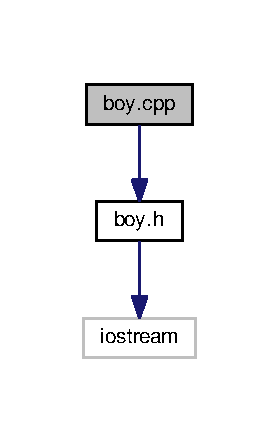
\includegraphics[width=134pt]{boy_8cpp__incl}
\end{center}
\end{figure}

\hypertarget{boy_8h}{}\section{boy.\+h File Reference}
\label{boy_8h}\index{boy.\+h@{boy.\+h}}
{\ttfamily \#include $<$iostream$>$}\\*
Include dependency graph for boy.\+h\+:
\nopagebreak
\begin{figure}[H]
\begin{center}
\leavevmode
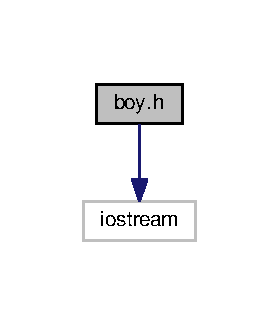
\includegraphics[width=134pt]{boy_8h__incl}
\end{center}
\end{figure}
This graph shows which files directly or indirectly include this file\+:
\nopagebreak
\begin{figure}[H]
\begin{center}
\leavevmode
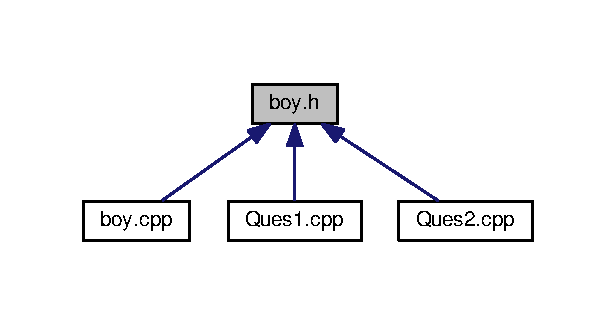
\includegraphics[width=295pt]{boy_8h__dep__incl}
\end{center}
\end{figure}
\subsection*{Classes}
\begin{DoxyCompactItemize}
\item 
class \hyperlink{classBoy}{Boy}
\end{DoxyCompactItemize}

\hypertarget{couple_8cpp}{}\section{couple.\+cpp File Reference}
\label{couple_8cpp}\index{couple.\+cpp@{couple.\+cpp}}
{\ttfamily \#include \char`\"{}couple.\+h\char`\"{}}\\*
Include dependency graph for couple.\+cpp\+:
\nopagebreak
\begin{figure}[H]
\begin{center}
\leavevmode
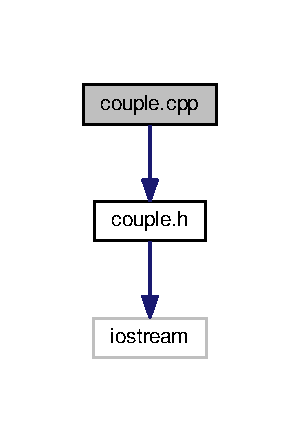
\includegraphics[width=144pt]{couple_8cpp__incl}
\end{center}
\end{figure}

\hypertarget{couple_8h}{}\section{couple.\+h File Reference}
\label{couple_8h}\index{couple.\+h@{couple.\+h}}
{\ttfamily \#include $<$iostream$>$}\\*
Include dependency graph for couple.\+h\+:
\nopagebreak
\begin{figure}[H]
\begin{center}
\leavevmode
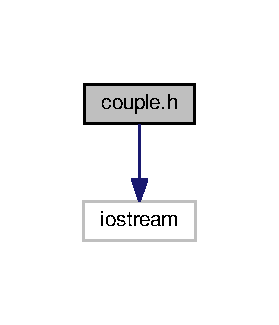
\includegraphics[width=134pt]{couple_8h__incl}
\end{center}
\end{figure}
This graph shows which files directly or indirectly include this file\+:
\nopagebreak
\begin{figure}[H]
\begin{center}
\leavevmode
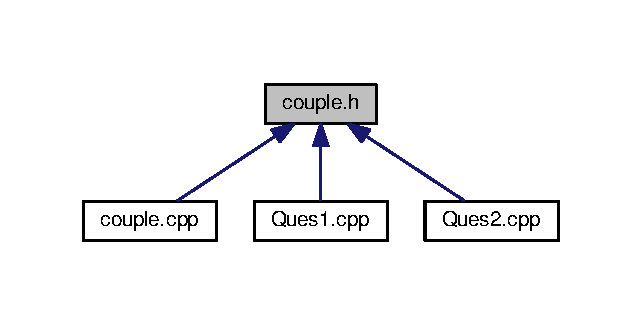
\includegraphics[width=308pt]{couple_8h__dep__incl}
\end{center}
\end{figure}
\subsection*{Classes}
\begin{DoxyCompactItemize}
\item 
class \hyperlink{classCouple}{Couple}
\end{DoxyCompactItemize}
\subsection*{Macros}
\begin{DoxyCompactItemize}
\item 
\#define \hyperlink{couple_8h_a5e0c07e523d4e77a2cafca06feb836f6}{Gf}~15
\end{DoxyCompactItemize}


\subsection{Macro Definition Documentation}
\index{couple.\+h@{couple.\+h}!Gf@{Gf}}
\index{Gf@{Gf}!couple.\+h@{couple.\+h}}
\subsubsection[{\texorpdfstring{Gf}{Gf}}]{\setlength{\rightskip}{0pt plus 5cm}\#define Gf~15}\hypertarget{couple_8h_a5e0c07e523d4e77a2cafca06feb836f6}{}\label{couple_8h_a5e0c07e523d4e77a2cafca06feb836f6}

\hypertarget{gift_8cpp}{}\section{gift.\+cpp File Reference}
\label{gift_8cpp}\index{gift.\+cpp@{gift.\+cpp}}
{\ttfamily \#include \char`\"{}gift.\+h\char`\"{}}\\*
Include dependency graph for gift.\+cpp\+:
\nopagebreak
\begin{figure}[H]
\begin{center}
\leavevmode
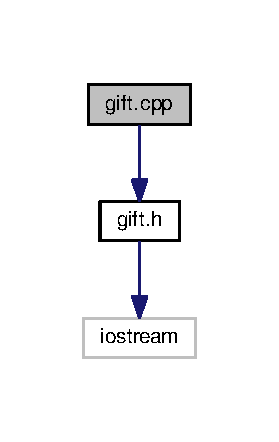
\includegraphics[width=134pt]{gift_8cpp__incl}
\end{center}
\end{figure}

\hypertarget{gift_8h}{}\section{gift.\+h File Reference}
\label{gift_8h}\index{gift.\+h@{gift.\+h}}
{\ttfamily \#include $<$iostream$>$}\\*
Include dependency graph for gift.\+h\+:
\nopagebreak
\begin{figure}[H]
\begin{center}
\leavevmode
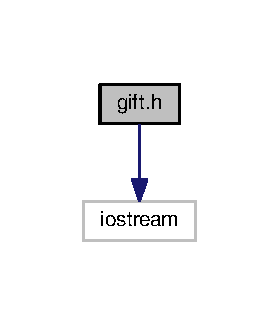
\includegraphics[width=134pt]{gift_8h__incl}
\end{center}
\end{figure}
This graph shows which files directly or indirectly include this file\+:
\nopagebreak
\begin{figure}[H]
\begin{center}
\leavevmode
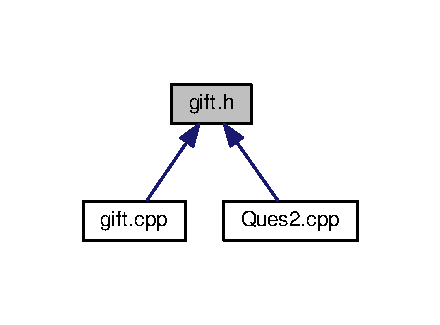
\includegraphics[width=211pt]{gift_8h__dep__incl}
\end{center}
\end{figure}
\subsection*{Classes}
\begin{DoxyCompactItemize}
\item 
class \hyperlink{classGift}{Gift}
\end{DoxyCompactItemize}

\hypertarget{girl_8cpp}{}\section{girl.\+cpp File Reference}
\label{girl_8cpp}\index{girl.\+cpp@{girl.\+cpp}}
{\ttfamily \#include \char`\"{}girl.\+h\char`\"{}}\\*
Include dependency graph for girl.\+cpp\+:
\nopagebreak
\begin{figure}[H]
\begin{center}
\leavevmode
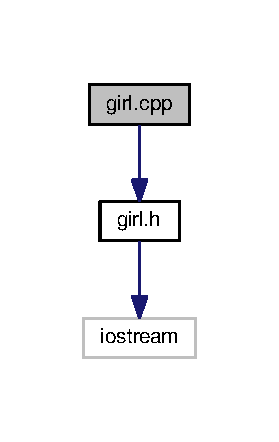
\includegraphics[width=134pt]{girl_8cpp__incl}
\end{center}
\end{figure}

\hypertarget{girl_8h}{}\section{girl.\+h File Reference}
\label{girl_8h}\index{girl.\+h@{girl.\+h}}
{\ttfamily \#include $<$iostream$>$}\\*
Include dependency graph for girl.\+h\+:
\nopagebreak
\begin{figure}[H]
\begin{center}
\leavevmode
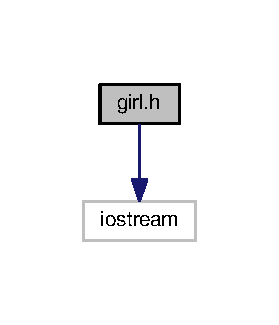
\includegraphics[width=134pt]{girl_8h__incl}
\end{center}
\end{figure}
This graph shows which files directly or indirectly include this file\+:
\nopagebreak
\begin{figure}[H]
\begin{center}
\leavevmode
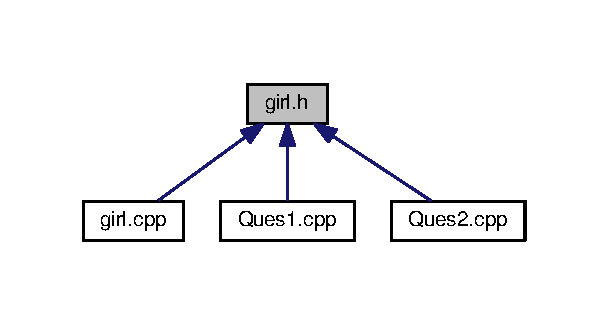
\includegraphics[width=292pt]{girl_8h__dep__incl}
\end{center}
\end{figure}
\subsection*{Classes}
\begin{DoxyCompactItemize}
\item 
class \hyperlink{classGirl}{Girl}
\end{DoxyCompactItemize}

\hypertarget{Ques1_8cpp}{}\section{Ques1.\+cpp File Reference}
\label{Ques1_8cpp}\index{Ques1.\+cpp@{Ques1.\+cpp}}
{\ttfamily \#include $<$iostream$>$}\\*
{\ttfamily \#include $<$fstream$>$}\\*
{\ttfamily \#include $<$sstream$>$}\\*
{\ttfamily \#include \char`\"{}boy.\+h\char`\"{}}\\*
{\ttfamily \#include \char`\"{}girl.\+h\char`\"{}}\\*
{\ttfamily \#include \char`\"{}couple.\+h\char`\"{}}\\*
Include dependency graph for Ques1.\+cpp\+:
\nopagebreak
\begin{figure}[H]
\begin{center}
\leavevmode
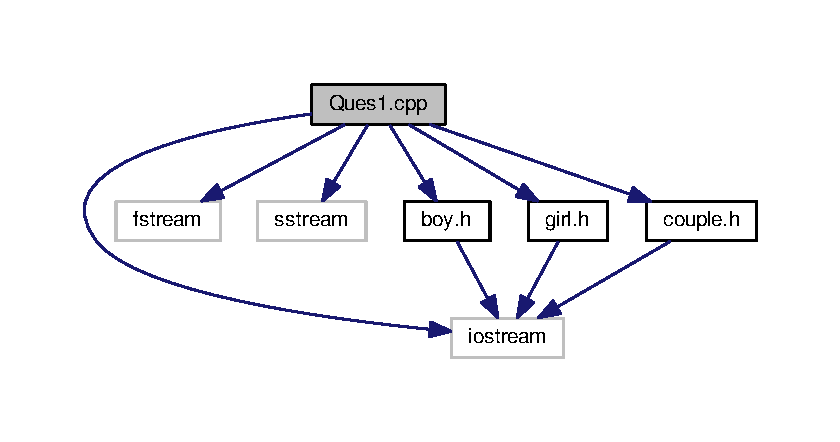
\includegraphics[width=350pt]{Ques1_8cpp__incl}
\end{center}
\end{figure}
\subsection*{Macros}
\begin{DoxyCompactItemize}
\item 
\#define \hyperlink{Ques1_8cpp_a111da81ae5883147168bbb8366377b10}{B}~5
\item 
\#define \hyperlink{Ques1_8cpp_aed9ea78689ecce0b7264c02c7f8a9a54}{G}~5
\item 
\#define \hyperlink{Ques1_8cpp_ac4cf4b2ab929bd23951a8676eeac086b}{C}~5
\end{DoxyCompactItemize}
\subsection*{Functions}
\begin{DoxyCompactItemize}
\item 
int \hyperlink{Ques1_8cpp_ae66f6b31b5ad750f1fe042a706a4e3d4}{main} ()
\end{DoxyCompactItemize}


\subsection{Macro Definition Documentation}
\index{Ques1.\+cpp@{Ques1.\+cpp}!B@{B}}
\index{B@{B}!Ques1.\+cpp@{Ques1.\+cpp}}
\subsubsection[{\texorpdfstring{B}{B}}]{\setlength{\rightskip}{0pt plus 5cm}\#define B~5}\hypertarget{Ques1_8cpp_a111da81ae5883147168bbb8366377b10}{}\label{Ques1_8cpp_a111da81ae5883147168bbb8366377b10}
\index{Ques1.\+cpp@{Ques1.\+cpp}!C@{C}}
\index{C@{C}!Ques1.\+cpp@{Ques1.\+cpp}}
\subsubsection[{\texorpdfstring{C}{C}}]{\setlength{\rightskip}{0pt plus 5cm}\#define C~5}\hypertarget{Ques1_8cpp_ac4cf4b2ab929bd23951a8676eeac086b}{}\label{Ques1_8cpp_ac4cf4b2ab929bd23951a8676eeac086b}
\index{Ques1.\+cpp@{Ques1.\+cpp}!G@{G}}
\index{G@{G}!Ques1.\+cpp@{Ques1.\+cpp}}
\subsubsection[{\texorpdfstring{G}{G}}]{\setlength{\rightskip}{0pt plus 5cm}\#define G~5}\hypertarget{Ques1_8cpp_aed9ea78689ecce0b7264c02c7f8a9a54}{}\label{Ques1_8cpp_aed9ea78689ecce0b7264c02c7f8a9a54}


\subsection{Function Documentation}
\index{Ques1.\+cpp@{Ques1.\+cpp}!main@{main}}
\index{main@{main}!Ques1.\+cpp@{Ques1.\+cpp}}
\subsubsection[{\texorpdfstring{main()}{main()}}]{\setlength{\rightskip}{0pt plus 5cm}int main (
\begin{DoxyParamCaption}
{}
\end{DoxyParamCaption}
)}\hypertarget{Ques1_8cpp_ae66f6b31b5ad750f1fe042a706a4e3d4}{}\label{Ques1_8cpp_ae66f6b31b5ad750f1fe042a706a4e3d4}

\hypertarget{Ques2_8cpp}{}\section{Ques2.\+cpp File Reference}
\label{Ques2_8cpp}\index{Ques2.\+cpp@{Ques2.\+cpp}}
{\ttfamily \#include $<$iostream$>$}\\*
{\ttfamily \#include $<$fstream$>$}\\*
{\ttfamily \#include $<$sstream$>$}\\*
{\ttfamily \#include $<$cmath$>$}\\*
{\ttfamily \#include \char`\"{}boy.\+h\char`\"{}}\\*
{\ttfamily \#include \char`\"{}girl.\+h\char`\"{}}\\*
{\ttfamily \#include \char`\"{}couple.\+h\char`\"{}}\\*
{\ttfamily \#include \char`\"{}gift.\+h\char`\"{}}\\*
Include dependency graph for Ques2.\+cpp\+:
\nopagebreak
\begin{figure}[H]
\begin{center}
\leavevmode
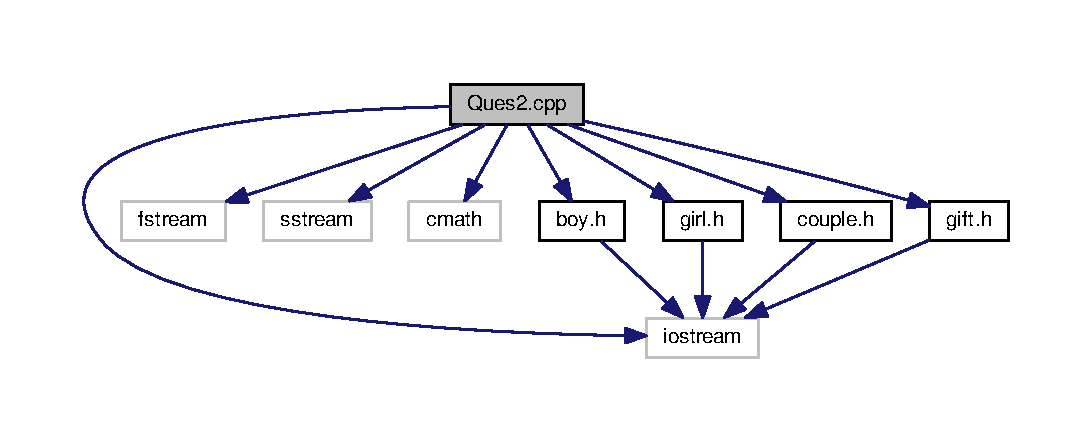
\includegraphics[width=350pt]{Ques2_8cpp__incl}
\end{center}
\end{figure}
\subsection*{Macros}
\begin{DoxyCompactItemize}
\item 
\#define \hyperlink{Ques2_8cpp_a111da81ae5883147168bbb8366377b10}{B}~5
\item 
\#define \hyperlink{Ques2_8cpp_aed9ea78689ecce0b7264c02c7f8a9a54}{G}~5
\item 
\#define \hyperlink{Ques2_8cpp_ac4cf4b2ab929bd23951a8676eeac086b}{C}~5
\item 
\#define \hyperlink{Ques2_8cpp_a5e0c07e523d4e77a2cafca06feb836f6}{Gf}~15
\item 
\#define \hyperlink{Ques2_8cpp_a97d832ae23af4f215e801e37e4f94254}{K}~3
\end{DoxyCompactItemize}
\subsection*{Functions}
\begin{DoxyCompactItemize}
\item 
void \hyperlink{Ques2_8cpp_ac70f752855ee1cf9ceaa2d749bbad17d}{swap} (\hyperlink{classGift}{Gift} \&a, \hyperlink{classGift}{Gift} \&b)
\item 
void \hyperlink{Ques2_8cpp_a9ed5e5ebda90f206f83cd424ebebe79d}{swapC} (\hyperlink{classCouple}{Couple} \&a, \hyperlink{classCouple}{Couple} \&b)
\item 
int \hyperlink{Ques2_8cpp_ae66f6b31b5ad750f1fe042a706a4e3d4}{main} ()
\end{DoxyCompactItemize}


\subsection{Macro Definition Documentation}
\index{Ques2.\+cpp@{Ques2.\+cpp}!B@{B}}
\index{B@{B}!Ques2.\+cpp@{Ques2.\+cpp}}
\subsubsection[{\texorpdfstring{B}{B}}]{\setlength{\rightskip}{0pt plus 5cm}\#define B~5}\hypertarget{Ques2_8cpp_a111da81ae5883147168bbb8366377b10}{}\label{Ques2_8cpp_a111da81ae5883147168bbb8366377b10}
\index{Ques2.\+cpp@{Ques2.\+cpp}!C@{C}}
\index{C@{C}!Ques2.\+cpp@{Ques2.\+cpp}}
\subsubsection[{\texorpdfstring{C}{C}}]{\setlength{\rightskip}{0pt plus 5cm}\#define C~5}\hypertarget{Ques2_8cpp_ac4cf4b2ab929bd23951a8676eeac086b}{}\label{Ques2_8cpp_ac4cf4b2ab929bd23951a8676eeac086b}
\index{Ques2.\+cpp@{Ques2.\+cpp}!G@{G}}
\index{G@{G}!Ques2.\+cpp@{Ques2.\+cpp}}
\subsubsection[{\texorpdfstring{G}{G}}]{\setlength{\rightskip}{0pt plus 5cm}\#define G~5}\hypertarget{Ques2_8cpp_aed9ea78689ecce0b7264c02c7f8a9a54}{}\label{Ques2_8cpp_aed9ea78689ecce0b7264c02c7f8a9a54}
\index{Ques2.\+cpp@{Ques2.\+cpp}!Gf@{Gf}}
\index{Gf@{Gf}!Ques2.\+cpp@{Ques2.\+cpp}}
\subsubsection[{\texorpdfstring{Gf}{Gf}}]{\setlength{\rightskip}{0pt plus 5cm}\#define Gf~15}\hypertarget{Ques2_8cpp_a5e0c07e523d4e77a2cafca06feb836f6}{}\label{Ques2_8cpp_a5e0c07e523d4e77a2cafca06feb836f6}
\index{Ques2.\+cpp@{Ques2.\+cpp}!K@{K}}
\index{K@{K}!Ques2.\+cpp@{Ques2.\+cpp}}
\subsubsection[{\texorpdfstring{K}{K}}]{\setlength{\rightskip}{0pt plus 5cm}\#define K~3}\hypertarget{Ques2_8cpp_a97d832ae23af4f215e801e37e4f94254}{}\label{Ques2_8cpp_a97d832ae23af4f215e801e37e4f94254}


\subsection{Function Documentation}
\index{Ques2.\+cpp@{Ques2.\+cpp}!main@{main}}
\index{main@{main}!Ques2.\+cpp@{Ques2.\+cpp}}
\subsubsection[{\texorpdfstring{main()}{main()}}]{\setlength{\rightskip}{0pt plus 5cm}int main (
\begin{DoxyParamCaption}
{}
\end{DoxyParamCaption}
)}\hypertarget{Ques2_8cpp_ae66f6b31b5ad750f1fe042a706a4e3d4}{}\label{Ques2_8cpp_ae66f6b31b5ad750f1fe042a706a4e3d4}
\index{Ques2.\+cpp@{Ques2.\+cpp}!swap@{swap}}
\index{swap@{swap}!Ques2.\+cpp@{Ques2.\+cpp}}
\subsubsection[{\texorpdfstring{swap(\+Gift \&a, Gift \&b)}{swap(Gift &a, Gift &b)}}]{\setlength{\rightskip}{0pt plus 5cm}void swap (
\begin{DoxyParamCaption}
\item[{{\bf Gift} \&}]{a, }
\item[{{\bf Gift} \&}]{b}
\end{DoxyParamCaption}
)}\hypertarget{Ques2_8cpp_ac70f752855ee1cf9ceaa2d749bbad17d}{}\label{Ques2_8cpp_ac70f752855ee1cf9ceaa2d749bbad17d}
\index{Ques2.\+cpp@{Ques2.\+cpp}!swapC@{swapC}}
\index{swapC@{swapC}!Ques2.\+cpp@{Ques2.\+cpp}}
\subsubsection[{\texorpdfstring{swap\+C(\+Couple \&a, Couple \&b)}{swapC(Couple &a, Couple &b)}}]{\setlength{\rightskip}{0pt plus 5cm}void swapC (
\begin{DoxyParamCaption}
\item[{{\bf Couple} \&}]{a, }
\item[{{\bf Couple} \&}]{b}
\end{DoxyParamCaption}
)}\hypertarget{Ques2_8cpp_a9ed5e5ebda90f206f83cd424ebebe79d}{}\label{Ques2_8cpp_a9ed5e5ebda90f206f83cd424ebebe79d}

%--- End generated contents ---

% Index
\backmatter
\newpage
\phantomsection
\clearemptydoublepage
\addcontentsline{toc}{chapter}{Index}
\printindex

\end{document}
